%% This is file `elsarticle-template-1-num.tex',
%%
%% Copyright 2009 Elsevier Ltd
%%
%% This file is part of the 'Elsarticle Bundle'.
%% ---------------------------------------------
%%
%% It may be distributed under the conditions of the LaTeX Project Public
%% License, either version 1.2 of this license or (at your option) any
%% later version.  The latest version of this license is in
%%    http://www.latex-project.org/lppl.txt
%% and version 1.2 or later is part of all distributions of LaTeX
%% version 1999/12/01 or later.
%%
%% The list of all files belonging to the 'Elsarticle Bundle' is
%% given in the file `manifest.txt'.
%%
%% Template article for Elsevier's document class `elsarticle'
%% with numbered style bibliographic references
%%
%% $Id: elsarticle-template-1-num.tex 149 2009-10-08 05:01:15Z rishi $
%% $URL: http://lenova.river-valley.com/svn/elsbst/trunk/elsarticle-template-1-num.tex $
%%
% \documentclass[preprint,review,12pt]{elsarticle}
\documentclass[final,3pd,times]{elsarticle}

%% Use the option review to obtain double line spacing
%% \documentclass[preprint,review,12pt]{elsarticle}

%% Use the options 1p,twocolumn; 3p; 3p,twocolumn; 5p; or 5p,twocolumn
%% for a journal layout:
%% \documentclass[final,1p,times]{elsarticle}
%% \documentclass[final,1p,times,twocolumn]{elsarticle}
%% \documentclass[final,3p,times]{elsarticle}
%% \documentclass[final,3p,times,twocolumn]{elsarticle}
%% \documentclass[final,5p,times]{elsarticle}
%% \documentclass[final,5p,times,twocolumn]{elsarticle}

%% if you use PostScript figures in your article
%% use the graphics package for simple commands
%% \usepackage{graphics}
%% or use the graphicx package for more complicated commands
%% \usepackage{graphicx}
%% or use the epsfig package if you prefer to use the old commands
%% \usepackage{epsfig}

%% The amssymb package provides various useful mathematical symbols
\usepackage{amssymb}
%\usepackage[T1]{fontenc}
%\usepackage[latin1]{inputenc}
\usepackage{graphicx}
\usepackage{listings}
\usepackage{url}
%% The amsthm package provides extended theorem environments
%% \usepackage{amsthm}

%% The lineno packages adds line numbers. Start line numbering with
%% \begin{linenumbers}, end it with \end{linenumbers}. Or switch it on
%% for the whole article with \linenumbers after \end{frontmatter}.
%% \usepackage{lineno}

%% natbib.sty is loaded by default. However, natbib options can be
%% provided with \biboptions{...} command. Following options are
%% valid:

%%   round  -  round parentheses are used (default)
%%   square -  square brackets are used   [option]
%%   curly  -  curly braces are used      {option}
%%   angle  -  angle brackets are used    <option>
%%   semicolon  -  multiple citations separated by semi-colon
%%   colon  - same as semicolon, an earlier confusion
%%   comma  -  separated by comma
%%   numbers-  selects numerical citations
%%   super  -  numerical citations as superscripts
%%   sort   -  sorts multiple citations according to order in ref. list
%%   sort&compress   -  like sort, but also compresses numerical citations
%%   compress - compresses without sorting
%%
%% \biboptions{comma,round}

% \biboptions{}

\lstset{keywordstyle=\bfseries,
  flexiblecolumns=true,
  showstringspaces=false,
  breaklines=true
}
\lstloadlanguages{[ANSI]C++,HTML}
\lstdefinestyle{prg} {basicstyle=\small\sffamily, showspaces=false}

\newcommand{\fig}[4][tbp]{
  \begin{figure}[#1]
    {\centering{\includegraphics[#4]{#2}}\par}
    \caption{#3}
    \label{fig:#2}
  \end{figure}
}

\newcommand{\Fig}[4][tbp]{
  \begin{figure*}[#1]
    {\centering{\includegraphics[#4]{#2}}\par}
    \caption{#3}
    \label{fig:#2}
  \end{figure*}
}

\newcommand{\class}[1]{{\sffamily\bfseries{#1}}}
\newcommand{\method}[1]{\class{#1}}
\newcommand{\us}{$\mu$s}
\newcommand{\ns}{$ns$}
\newcommand{\ms}{$ms$}

\journal{Computers and Electrical Engineering}

\begin{document}

\begin{frontmatter}

%% Title, authors and addresses

%% use the tnoteref command within \title for footnotes;
%% use the tnotetext command for the associated footnote;
%% use the fnref command within \author or \address for footnotes;
%% use the fntext command for the associated footnote;
%% use the corref command within \author for corresponding author footnotes;
%% use the cortext command for the associated footnote;
%% use the ead command for the email address,
%% and the form \ead[url] for the home page:
%%
%% \title{Title\tnoteref{label1}}
%% \tnotetext[label1]{}
%% \author{Name\corref{cor1}\fnref{label2}}
%% \ead{email address}
%% \ead[url]{home page}
%% \fntext[label2]{}
%% \cortext[cor1]{}
%% \address{Address\fnref{label3}}
%% \fntext[label3]{}

\title{Periodic Timers Revisited: the Real-time Embedded System Perspective\tnoteref{Grant}}
\fntext[Grant]{This work was partially supported by the Coordination for Improvement of Higher Level Personnel (CAPES) grant, projects RH-TVD 006/2008 and 240/2008.}

%% use optional labels to link authors explicitly to addresses:
%% \author[label1,label2]{<author name>}
%% \address[label1]{<address>}
%% \address[label2]{<address>}

\author{Ant\^{o}nio Augusto Fr\"{o}hlich\corref{cor1}}
\ead{guto@lisha.ufsc.br}
\author{Giovani Gracioli}
\ead{giovani@lisha.ufsc.br}
\author{Jo\~{a}o Felipe Santos}
\ead{jfsantos@lisha.ufsc.br}

\address{Software/Hardware Integration Lab, Federal University of Santa
  Catarina, 88040-900 Florian\'{o}polis - SC, Brazil }

\cortext[cor1]{Corresponding author. Tel./Fax: +55 48 3721 9516}

% 145 words - Should be between 100 and 150
\begin{abstract}
  Common sense dictates that single-shot timer mechanisms are more
  suitable for real-time applications than periodic ones, specially in
  what concerns precision and jitter. Nevertheless, \emph{real-time
    embedded systems} are inherently periodic, with tasks whose periods
  are almost always known at design-time. Therefore a carefully designed
  periodic timer should be able to incorporate much of the advantages of
  single-shot timers and yet avoid hardware timers reprogramming, an
  expensive operation for the limited-resource platforms of typical
  embedded systems.

  In this paper, we describe and evaluate two timing mechanisms for
  embedded systems, one periodic and another single-shot, aiming at
  comparing them and identifying their strengths and weaknesses.  Our
  experiments have shown that a properly designed periodic timer can
  usually match, and in some cases even outperform, the single-shot
  counterpart in terms of precision and interference, thus
  reestablishing periodic timers as a dependable alternative for
  real-time embedded systems.
\end{abstract}

\begin{keyword}
%% keywords here, in the form: keyword \sep keyword

%% MSC codes here, in the form: \MSC code \sep code
%% or \MSC[2008] code \sep code (2000 is the default)
Real-time Operating System \sep
Operating System Time Management \sep
Single-shot Timer
\end{keyword}

\end{frontmatter}

%%
%% Start line numbering here if you want
%%
% \linenumbers

%% main text
\section{Introduction} \label{sec:intro}

% - What is timing about?
% - How timing has been done in ordinary OS?
The notion of time is essential to any real-time embedded system. The
system needs to keep track of time flow to schedule tasks and also to
provide time services, such as delays and alarms, to applications.
Historically, operating systems (OS) have been implementing time
management based on a hardware timer that is configured to periodically
trigger interrupts, thus giving rise to a system time unit called
\emph{tick}. Ticks define the minimum perception of time flow within the
system and rule every sort of time-driven events. The mechanism is
usually implemented with a single hardware timer, whose interrupt
handler is overloaded with operations around task scheduling and timed
event propagation.

% - Criticize periodic timer and introduce single-shot
Though well-accepted in the realm of general-purpose systems, time
management strategies based on periodic timers face strong criticism
from the real-time system community~\cite{Tsafrir:2005}. For instance,
in a system with a periodic timer configured to generate 10~\ms{} ticks,
a 15~\ms{} delay request may result, in the worst case, in a waiting
time of 30~\ms{}. Figure~\ref{fig:worst_case_periodic_timer} exemplifies
this worst-case scenario. The request is posted just after a tick is
generated, thus counting will only start on the next tick. Moreover, 15
might be rounded up to 20 (multiple of a tick), yielding a total time of
30~\ms. In addition to the lack of precision in time services, the
periodic timer handler is constantly activated, even if no action needs
to be taken, causing overhead and interference on running tasks.  These
limitations fostered the mechanism of \emph{single-shot} timer, with
dedicated timers being programmed to fire exactly when an action has to
be performed~\cite{Tsafrir:2005,Aron:2000,Goel:2002}.

\fig{worst_case_periodic_timer}{An example of a worst case scenario for
  a delay request using a periodic timer.}{scale=.6}

% - Rescue periodic timer
Nonetheless, despite these unquestionable issues about periodic timers,
while performing experiments in the context of a previous
paper~\cite{Gracioli2008}, we realized that single-shot supremacy might
be indeed more closely connected to implementation issues than to the
concept itself. Some of the aspects that called our attention were:

\begin{itemize}
\item Real-time embedded systems are intrinsically periodic. Even simple
  software architectures, such as cyclic executives, have a period
  derived from the main loop length. Real-time scheduling in more
  complex embedded systems is essentially periodic (e.g., Earliest
  Deadline First, Rate Monotonic, etc).

\item Single-shot timers are usually multiplexed on a few physical
  timers, demanding constant hardware reprogramming, what, in some
  systems is much slower than software reprogramming.

\item Single-shot timers, in practice, do overflow, demanding some sort
  of periodic fall-back mechanism.
\end{itemize}

In this way, a carefully designed periodic timer mechanism could, in
theory, incorporate much of the advantages of single-shot timers.
Indeed, even non real-time OS now feature improved periodic timers:
\textsc{Windows Vista} can adjust the period of the hardware timer
according to the system load~\cite{Peter:2008}; \textsc{Linux} delivers
a secondary high resolution timing interface to
applications~\cite{Siddha:2007}.  Therefore, in this paper we
investigated this hypothesis by comparing the behavior of both time
management strategies (i.e., periodic and single-shot) in the same
scenario (i.e., hardware platform, OS, and applications). Our results
confirmed that a properly configured and implemented periodic timer may
yield high precision and low overhead.  Single-shot timers, on the other
hand, are usually able to match the precision of periodic timers, and
can cause less interference in the system when a periodic timer is not
well-configured. The design and implementation considerations presented
in this paper can be incorporated by virtually any OS. They can also
serve as guidelines for other groups developing single-shot timer
mechanisms on the premise that this would eliminate all the trouble
caused by periodic timers on real-time applications.

The remainder of this paper is organized as follows:
section~\ref{sec:rel} presents related work; section~\ref{sec:design}
presents the design and implementation of single-shot and periodic
timing mechanisms; section~\ref{sec:case} describes the experimental
evaluation of proposed mechanisms, along with a comparative analysis;
section~\ref{sec:con} closes the paper with our final considerations.

\section{Related Work}\label{sec:rel}

Tsafrir, Etsion, and Feitelson approach some important issues around
periodic time management, particularly lack of precision and power
consumption, as they introduced the concept of \emph{Smart
  Timer}~\cite{Tsafrir:2005}. The proposed timer mechanism can be
summarized by three main properties: 1) Accurate timing with configurable
maximum latency; 2) Reduced management overhead by triggering combined
nearby events, and (3) Reduced overhead by avoiding unnecessary periodic
events.

Kohout presents a strategy to efficiently support RTOS using core
components implemented in hardware~\cite{Kohout:2003}. The main
objective is to reduce the impact caused by the RTOS on applications,
which is assessed in terms of response time and CPU usage. The work
introduces the Real-Time Task Manager (RTM), a hardware component that
deals with task scheduling, time management, and event management. The
RTM support for time management functions causes a 10\% reduction on CPU
time (with 24 tasks).

Aron and Druschel introduced the concept of \emph{Soft-Timer}, which
triggers the time manager on the return of every system
call~\cite{Aron:2000}. Hardware timer interrupts are simultaneously
deployed to ensure minimum timing requirements for applications.  Their
measurements show a reduction in the number of context switches and an
increase in the time service precision. This is mainly attributed to the
fact that system calls tend to be more frequent than timer interrupts.
Nonetheless, periodic timer interrupts are still necessary, since the
rate of system calls is unpredictable.

\emph{Firm Timer} combines three different time management approaches,
single-shot timer, soft-timer, and periodic timer, to build an
efficient, high-resolution, low-overhead mechanism~\cite{Goel:2002}. The
mechanism uses an "overshooting" parameter S, that is added in a
requested time T (T + S).  If the kernel is called by a system call,
interrupt, or an exception after T, but before T + S, then the requested
period is handled (\emph{Soft-Timer} approach), and the overhead
associated to the interrupt handler at T + S is avoided. The authors
claim that in some cases the kernel is called after a timer has expired
but before the timer generates an interrupt. The combination of the
three time management approaches allows a reduction in the number of
timer interrupts, thus reducing the overall overhead of periodic timers
in the system. However, as in the \emph{Soft-Timer}, there is an extra
overhead associated to polling and checking for timers at each
soft-timer point~\cite{Goel:2002}. Moreover, the overshooting parameter
causes a lack of timing precision, which compromises its use in
hard-real time applications.

\textsc{L4-embedded} microkernel implements time management using a
traditional periodic timer scheme, but exempts the interrupt handler
from duties such as time-out management and time-of-day keeping. Those
activities are performed by specific servers at user-level. This work
distribution improves the response time of the interrupt
handler~\cite{Ruocco:2008}.  Single-shot timer mechanisms are to be used
in future versions of the system aiming at energy consumption
optimization.

Several groups have proposed modification in the time management
strategy of \textsc{Linux} focusing on (soft) real-time applications.
\textsc{UTIME} was one the first projects to investigate how
high-resolution timers could be implemented in
\textsc{Linux}~\cite{Srinivasan:98}. The main timer is reprogrammed to
trigger interrupts on a single-shot manner. A secondary hardware device,
similar to the time-stamp counter on x86-based machines, is used to keep
the elapsed time counter. Since both timers have quite distinct
resolutions, the approach reduces interference at the risk of precision
loss (due to conversions between both devices).  Stultz and Hart
proposed a significant re-work in the \textsc{Linux} timing subsystem by
changing its internal structures and interfaces~\cite{Stultz:2006}.  The
new internal structures and interfaces were designed facing nanoseconds,
instead of ticks. Moreover, the existing interfaces continue to be
supported, although they are less precise. \textsc{Hrtimer} is another
abstraction in the \textsc{Linux} timing subsystem proposed by Gleixner
and Niehaus~\cite{Gleixner:2006}. It explores recently added timing
devices (e.g. \emph{High-Precision Event Timer} on x86-based PCs) to
implement high-resolution time events specified in nanoseconds (not in
ticks).  Time events are kept in a per-CPU red-black tree ordered by the
absolute expiration time and are handled independently from tick-based
time events.

Regarding time management in Real-Time Operating Systems (RTOS),
\textsc{QNX Neutrino} provides a set of POSIX timer interface, therefore
time may be measured in nanoseconds or seconds~\cite{QNX}. The time
management is based on periodic timer.  A process can sleep or delay its
execution by using absolute time (timer contains the current Coordinated
Universal Time (UTC) relative to January 1, 1970) or relative to the
current clock value. Moreover, a process can also control the timer
resolution by using the concept of \emph{ticksize}, which can have a
resolution from 500 microseconds to 50 milliseconds.
\textsc{RTLinuxFree}~\cite{RTLinuxFree},
\textsc{Xenomai}~\cite{Xenomai}, and \textsc{RTAI}~\cite{Cloutier:00}
are real-time extensions to the \textsc{Linux} kernel.
\textsc{RTLinuxFree} treats the \textsc{Linux} kernel as an idle task,
executing it when there are no real-time tasks ready to run. All
interrupts are handled by \textsc{RTLinuxFree} micro-kernel. It can
respond to an interrupt no matter whether \textsc{Linux} does (for
example, executing a spin-lock or disabling/enabling interrupts).
\textsc{RTLinuxFree} supports both periodic and single-shot timer
operating modes~\cite{Kairui:2006}.  \textsc{Xenomai} and \textsc{RTAI}
use the \textsc{Adeos} nanokernel~\cite{Karim:2001}, which is
responsible for handling the hardware interrupts. \textsc{Adeos}
forwards a received interrupt to \textsc{Xenomai}/\textsc{RTAI} to be
properly handled before the \textsc{Linux}, that is,
the RTOS has a higher priority in relation to \textsc{Linux}. Both \textsc{Xenomai} and
\textsc{RTAI} offer support for periodic and one-shot time management.
\textsc{VxWorks} is the most widely adopted commercial RTOS in the
embedded industry~\cite{VxWorks}. This RTOS also implements the POSIX
timer interface and its time management is based on periodic timers.

In summary, all these works focus on eliminating the side-effects
associated to the maintenance of a global system's tick counter.  In
particular, activation of the timer interrupt handler solely to
increment the tick counter is strongly avoided. For this purpose,
single-shot mechanisms are proposed. The performance evaluation of such
mechanisms, however, is mostly done in the context of general-purpose
systems, disregarding hardware reconfiguration times and the periodic
nature of real-time embedded systems.


\section{Design and Implementation} \label{sec:design}

The design and implementation of the single-shot timer and periodic
timer were carried out in the Embedded Parallel Operating System
(\textsc{Epos}\footnote{\textsc{Epos} is available online at
  \url{http://epos.lisha.ufsc.br}.})~\cite{Froehlich:2001}.
\textsc{Epos} is a multi-platform, component-based, embedded system
framework in which traditional OS services are implemented through
adaptable, platform-independent \emph{System Abstractions}.
Platform-specific support is implemented through \emph{Hardware
  Mediators}~\cite{Polpeta:2004}, which are functionally equivalent to
device drivers in \textsc{Unix}, but do not build a traditional HAL.
Instead, they sustain the interface contract between abstractions and
hardware components by means of static metaprogramming techniques that
``dilute'' mediator code into abstractions at compile-time (no calls, no
layers, no messages; mostly embedded assembly). This is the main reason
why we decided to conduct our timing experiments with \textsc{Epos}: the
small and clean executable code produced by the framework enabled us to
directly assess secondary sources of interference which were
subsequently eliminated.

Time is managed in \textsc{Epos} by the families of components shown in
Figure~\ref{fig:epos_time}. The \class{Clock} abstraction is responsible
for keeping track of the current time, and is only available on systems
that feature a real-time clock device, which is in turn abstracted by a
member of the \class{RTC} family of mediators.  The \class{Chronometer}
abstraction is used to measure time intervals, through the use of a
timestamp counter (\class{TSC}) mediator. If a given platform does not
feature a hardware TSC, its functionality may be emulated by an ordinary
periodic timer.

\fig[bht]{epos_time}{\textsc{Epos} timing components.}{scale=.6}

The \class{Alarm} abstraction can be used to generate timed events, and
also to put a thread to \emph{sleep} for a certain time.  For this
purpose, an application instantiates a handler and registers it with an
Alarm specifying a time period and the number of times the handler
object is to be invoked. \textsc{Epos} allows application processes to
handle events at user-level through the \class{Handler} family of
abstractions depicted in Figure~\ref{fig:epos_handler}. The
\class{Handler\_Function} member assigns an ordinary function supplied
by the application to handle an event. The \class{Handler\_Thread}
member assigns a thread to handle an interrupt. Such a thread must have
been previously created by the application in the suspended state. It is
then resumed at every occurrence of the corresponding event. Finally,
the \class{Handler\_Semaphore} assigns a semaphore, previously created
by the application and initialized with zero, to an event. The OS
invokes operation \method{v} on this semaphore at every event
occurrence, while the handling thread invokes operation \method{p} to
wait for an event. Although not in the scope of this work, it is worth
to mention that the same mechanisms are used in \textsc{Epos} for
real-time thread scheduling~\cite{Marcondes:2009}.
 %Figure~\ref{prg:time_app} illustrates how an application uses time services in the \textsc{Epos} system.

\fig[bht]{epos_handler}{\textsc{Epos} event handlers.}{scale=.6}

The \class{Timer} class abstracts timing hardware.  In a periodic event
model, the platform's timer is set with a constant (configurable)
frequency. When a new alarm event is registered, its interval is
converted to timer \emph{ticks}, with $ T = \frac{I}{F} $, where $T$ is
the number of ticks, $I$ is the desired interval, and $F$ is the timer
frequency. The event is then inserted into an ordered and relative
request queue. Thus, manipulation of this queue affects only its head,
because it keeps all values relative to the first element.  Due to
rounding errors, the number of ticks may not correspond to the exact
desired interval. When a timer interrupt is triggered, an interrupt
handler, registered by the \class{Alarm} abstraction, increments the
tick counter, thus promoting every alarm in the event queue by a tick.
If the event at the head of the queue has no more ticks to count, its
handler is released. The corresponding interrupt handler is depicted in
the Unified Modeling Language (UML) sequence diagram of
Figure~\ref{fig:handlers}(a).

%\fig{handler_periodic}{Periodic alarm handler sequence diagram.}{scale=.3}

\begin{figure*}[ht]
\centering
\begin{tabular}{cc}
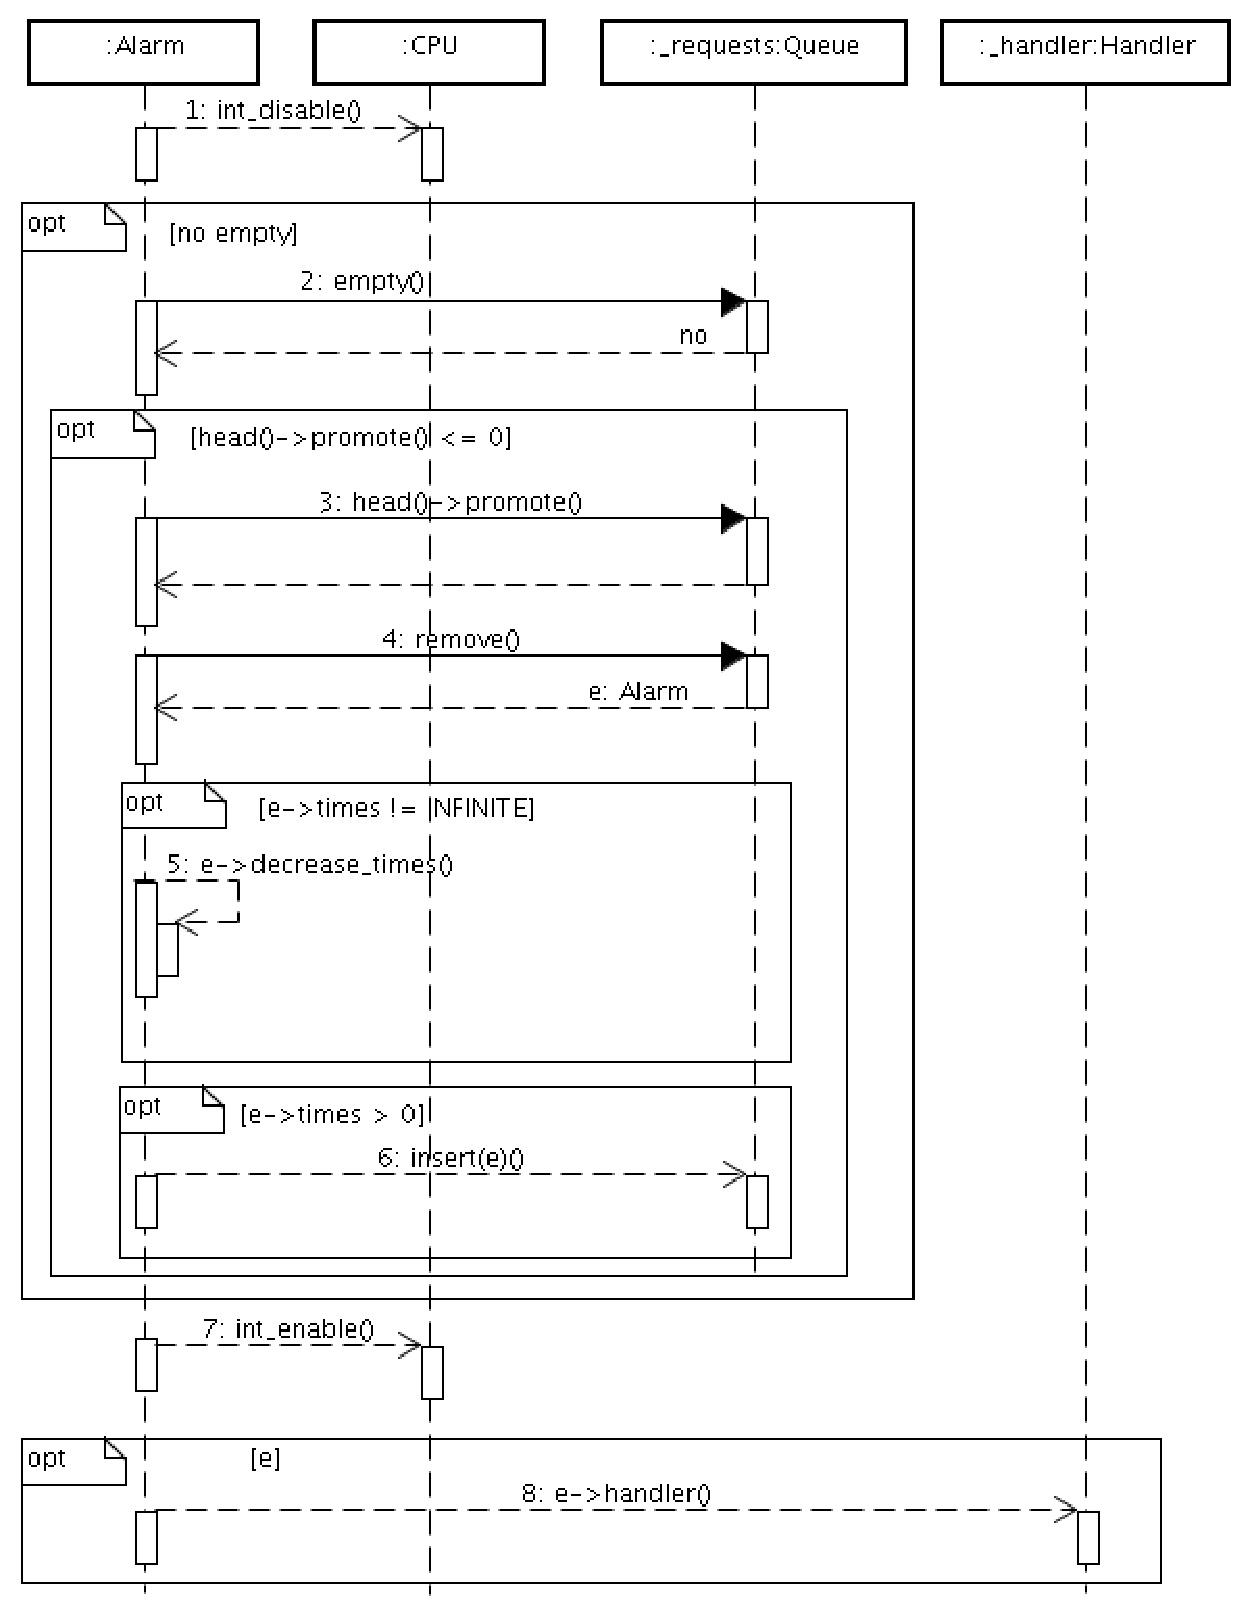
\includegraphics[width=0.4\columnwidth]{handler_periodic} &
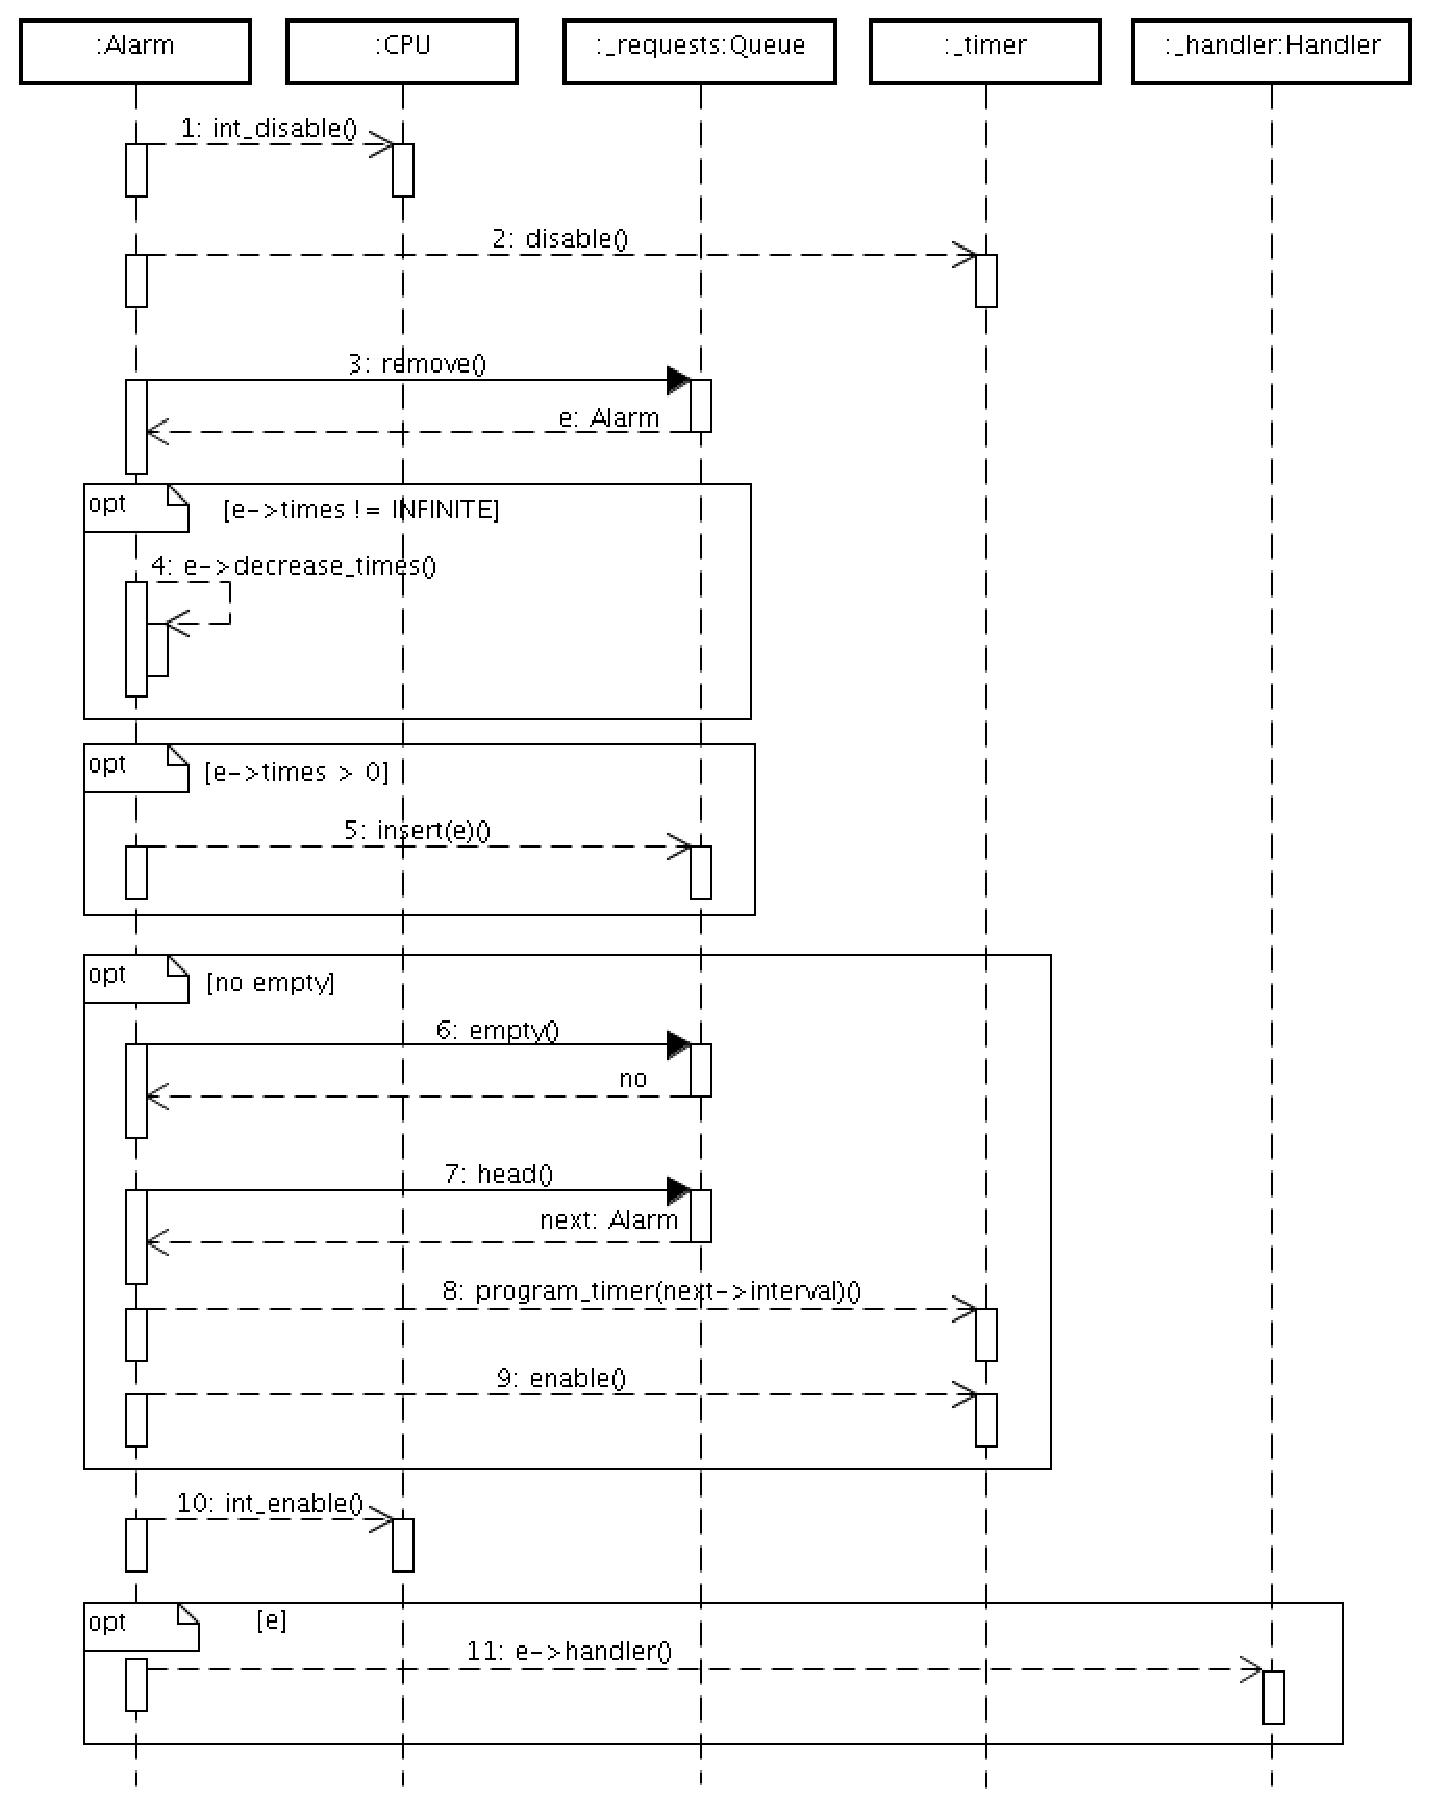
\includegraphics[width=0.41\columnwidth]{handler_single-shot}\\
(a)  & (b) \\
\end{tabular}
\caption{(a) Periodic alarm handler sequence diagram (b) Single-shot
  alarm handler sequence diagram.}
\label{fig:handlers}
\end{figure*}

Figure~\ref{fig:class_diagram} presents the class diagram of
\class{Alarm} and \class{Chronometer} abstractions for the AVR-8
architecture~\cite{atmega128datasheet}. The \class{Alarm} abstraction
uses two of the hardware timers available in the AVR microcontroller.
One of these timers, \class{ATMega128\_Timer\_3}, is used to control the
\class{Alarm} request queue. With the system clock configured at 7.2 MHz
and a prescale of 1024, this 16-bit timer allows the scheduling of
events spanning approximately 9 seconds.  The other timer,
\class{ATMega128\_Timer\_1}, generates periodic interrupts that trigger
the system scheduler. These interrupts only occur when the scheduler is
active, with a period that corresponds to the system's configured
\emph{quantum}.

\fig[ht]{class_diagram}{Class diagram of \textsc{Epos} abstractions and
  mediators for the AVR-8 architecture.}{scale=.41}

Figure~\ref{prg:time_app} illustrates how an application uses time
services in the \textsc{Epos} system. This application reads current
system time through a \class{Clock} object, measures time intervals with
a \class{Chronometer}, and registers a periodic \class{Alarm} with an
associated \class{Handler\_Function}.

\begin{figure}[ht]
   \lstset{frame=single,language=C++,xleftmargin=2em,style=prg,basicstyle=\scriptsize}
   \begin{lstlisting}
static int iterations = 100;
static Alarm::Microsecond time = 100000;
int main() 
{
    OStream cout;
    Clock clock;
    Chronometer chron;
    // Read current system time
    cout << "Current Time: " << clock.now() << endl;
    // Create a handler function and associate it to a periodic time event
    Handler_Function handler(&func);
    Alarm alarm(time, &handler, iterations);
    // Start a chronometer and put this thread to sleep. Afterwards, stop and read the chronometer
    chron.start();
    Alarm::delay(time * (iterations + 1));
    chron.stop();
    cout << "Elapsed time: " << chron.read() << endl;
    return 0;
}    
   \end{lstlisting}
  \caption{Example of time service utilization in \textsc{Epos}.}
  \label{prg:time_app}
\end{figure}

In this work, we designed and implemented a new event model, based on
\emph{single-shot} timers. In a single-shot model, the platform's timer
is programmed based on the interval to the next event. New events are
enqueued according to their relative interval order.  The \class{Alarm}
interrupt handler promotes every alarm in the event queue with the time
elapsed since the last interrupt, and reprograms the timer with the next
event's interval. Since in this scheme there are no conversions between
intervals and ticks, precision loss is restricted to physical timer
resolution.

In order to generate interrupts at a given frequency, hardware timers
are usually configured with a frequency prescaler (relative to processor
clock), and a comparison register. The hardware timer counts a tick at
each clock period, and triggers an interrupt when the ticks counter
reaches the value in the comparison register.  Valid hardware periods
are given by the following equation:

\begin{equation}
\frac{D}{C}  \leq  P \leq  \frac{D \times (2^{r} - 1)}{C} 
\label{eq:period}
\end{equation}

\noindent where $D$ is the clock prescaler, $C$ is the system's clock
frequency, $P$ is the timer's period, and $r$ is the timer's resolution.
Thus, when the desired event interval is larger than the timer's
hardware resolution, the \class{Timer} mediator needs to count ticks in
software.

In order to allow waiting for a period larger than the hardware timer
resolution, without incurring in overhead when this is not necessary, we
introduced a \method{MAX\_PERIOD} \emph{configuration trait} to the
timer implementation. This trait allows compile-time specialization for
either hardware or software based counting, as necessary. When software
counting is activated, the \class{Timer} mediator handles its own
interrupt, in which it increments a tick counter. When this counter is
equal to the desired period, a new interrupt is triggered by the
software, to be handled by the \class{Alarm} abstraction. As was the
case with periodic timers, there may be rounding errors introduced by
the conversion from period to ticks. Since the interrupt to be handled
by the \class{Alarm} changes according to configuration, the timer
informs its interrupt request (IRQ) through a class method.  The
corresponding interrupt handler is depicted in the UML sequence diagram
of Figure~\ref{fig:handlers}(b).

%\fig{handler_single-shot}{Single-shot alarm handler sequencediagram.}{scale=.3}

\section{Experimental Evaluation}\label{sec:case}

In order to evaluate the proposed time management strategies, we devised
some experiments. Our first experiment was targeted at measuring the
actual period of events with distinct periods, in different timer clock
configurations.  Figure~\ref{prg:alarm} presents the application
implemented for this test. The main thread creates an alarm event with
several iterations, and waits for the completion of all handlers. For
each test, the period of each event was configured with a different
value, from 100~$\mu$s to 10~s. Each event handler stores the timestamp
of its execution instant. The difference between two consecutive
timestamps results in an interval that, ideally, should be equal to the
requested event period.

\begin{figure}[bht]
   \lstset{frame=single,language=C++,xleftmargin=2em,style=prg,basicstyle=\scriptsize}
   \begin{lstlisting}
static Chronometer chron;
static Microsecond time_stamps[11];
volatile static int n = 0;
void handler(void) { time_stamps[n++] = chron.read(); }
int main() {
    // Register the events
    Handler_Function handler(&handler);
    Alarm alarm(PERIOD, &handler, 11);
    // Wait for all handlers to finish
    while(n<11) {  }
    // Print intervals
    for(unsigned int i = 0; i < 10; i++)
	cout << time_stamps[i+1] - time_stamps[i] << endl;
}
   \end{lstlisting}
  \caption{Periodic alarm application.}
  \label{prg:alarm}
\end{figure}

For every period and clock frequency, the periodic timer's frequency,
and the single-shot timer's maximum period were configured with
\emph{ideal} values. Thus, for example, if the event's period was 1~s,
the periodic timer's frequency was set to 1~Hz, and single-shot timer's
maximum period was set to 1~s. From this follows that, whenever
possible, the periodic timer's behavior was equivalent to that of a
single-shot timer: the timer's interrupt is only triggered when there is
an event to run. Likewise, the single-shot timer's implementation only
falls back to software tick counting when strictly necessary (i.e. when
the requested event period is larger than the hardware's resolution).
Thus, our tests yield the best possible results for each timing
strategy.

We executed this experiment in an 8-bit AVR microcontroller (ATMega128),
with a 16-bit timer/counter~\cite{atmega128datasheet}.  We configured
this timer with three different clock frequencies: 7200~Hz, 28800~Hz,
and 115200~Hz.  Tables~\ref{tab:error_periodic}
and~\ref{tab:error_single-shot} present the average total period of each
event, configured with different clock frequencies, in each timing
strategy. It should be noted that, while the single-shot timing strategy
usually presents better results than its periodic equivalents, both
strategies present considerable errors for short periods when a ``slow''
(e.g. 7200~Hz) timer clock is used. Furthermore, when the requested
period exceeds the maximum hardware period, and the single-shot timer
falls back to software tick counting, errors for this strategy increase
considerably. Likewise, when using a very ``fast'' (e.g. 115200~Hz)
timer clock, the overhead of reprogramming the single-shot timer may
exceed the overhead of counting ticks in periodic timers. Finally, it
should be noted that these values represent a best-case scenario for
periodic timers, since the timer's period was configured as close to the
event's period as possible. Nonetheless, these values represent a
typical case for single-shot timers whenever the maximum event period is
smaller or equal to the maximum timer hardware period.

\begin{table}[ht]
\centering
\scriptsize{
\begin{tabular}{c|c|c|c}
\multicolumn{4}{c}{\textbf{Periodic Timer Period (us)}} \\
\hline
\textbf{Requested}	& \multicolumn{3}{c}{\textbf{Measured}} \\
\cline{2-4}
\textbf{Period}	& \textbf{7200 Hz}	& \textbf{28800 Hz} 	& \textbf{115200 Hz} \\
\hline
\textbf{100}		& 277		& 173		& 147		\\
\textbf{1.000}		& 1.944		& 1.214		& 1.032		\\
\textbf{10.000}		& 10.138	& 10.034	& 10.008	\\
\textbf{100.000}	& 100.138	& 100.034	& 100.008	\\
\textbf{1.000.000}	& 1.000.138	& 1.000.034	& 1.000.016	\\
\textbf{10.000.000}	& 10.001.388	& 10.000.346	& 10.000.173	\\
\end{tabular}
}
\caption{Difference between expected and measured periods using periodic timer.}
\label{tab:error_periodic}
\end{table}

\begin{table}[ht]
\centering
\scriptsize{
\begin{tabular}{c|c|c|c}
\multicolumn{4}{c}{\textbf{Single-Shot Timer Period (us)}} \\
\hline
\textbf{Requested}	& \multicolumn{3}{c}{\textbf{Measured}} \\
\cline{2-4}
\textbf{Period}	& \textbf{7200 Hz}	& \textbf{28800 Hz} 	& \textbf{115200 Hz} \\
\hline
\textbf{100}		& 268		& 164		& 136		\\
\textbf{1.000}		& 1.240		& 1.031		& 1.031		\\
\textbf{10.000}		& 10.128	& 10.059	& 10.033	\\
\textbf{100.000}	& 100.128	& 100.059	& 100.036	\\
\textbf{1.000.000}	& 1.000.128	& 1.000.094	& 1.152.970	\\
\textbf{10.000.000}	& 10.138.457	& 10.282.728	& 10.921.704	\\
\end{tabular}
}
\caption{Difference between expected and measured periods using single-shot timer.}
\label{tab:error_single-shot}
\end{table}

Figure~\ref{fig:error} presents error curves (actual period relative to
ideal period) for each tested period, in each clock configuration, for
each timing strategy. In every case, the error rates decrease as the
requested period increases, and as the timer's clock speed increases.
With larger periods and faster timer clocks, the overhead and rounding
errors of the timing system are minimized. The upwards slope in the
single-shot tests represents the moment where the timer's hardware
maximum period is exceeded, and the timer falls back on software tick
counting.

\fig[ht]{error}{Error rates for different periods.}{scale=0.65}

While a periodic timer may have equivalent or even superior performance
than a single-shot timer, its implementation may interfere with other
parts of the system. A single-shot timer only generates interrupts when
there is an event to be handled, while a periodic timer generates
interrupts at a constant rate, regardless of whether there is an event
to handle or not.  Thus, a periodic timer service may interfere with
other threads in the system. In order to evaluate this phenomenon, we
measured the time spent in handling an alarm event in both approaches
using the same AVR platform. At the beginning of the alarm handler, we
turned a LED on and before leaving the handler we turned it off. We
connected a digital oscilloscope to the output of the LED to measure the
elapsed time.  For this test, an alarm triggered at every 5~ms and the
timer was configured with a frequency of 1000~Hz and a clock of
125000~Hz. A periodic timer generates four interrupts before the alarm
is released, that is, during 4 interrupts it will only count ticks.  The
single-shot timer only triggers when it is necessary, but it must
reprogram the timer after each event. The goal of the experiment is to
measure the interference of both approaches in the system as a whole.
Obtained values are shown in Table~\ref{tab:handler_time}.  For an
interrupt that counts ticks, the periodic timer took 14~\us{} and for an
interrupt where is necessary to release the alarm it took 42~\us{}.  The
single-shot timer, however, took 212~\us{} for releasing the alarm
event. This high overhead is due to the time needed to reprogram the
hardware timer.

\begin{table}[bht]
\centering
\scriptsize{
\begin{tabular}{c|c|c}
\textbf{Interrupt / Approach} & \textbf{Periodic} & \textbf{Single-Shot} \\
\hline
Counting ticks interrupt & 14~\us{} & - \\
Alarm release interrupt  & 42~\us{} & 212~\us{} \\
\end{tabular}
}
\caption{Time spent in handling the alarm interrupt using periodic and single-shot timers.}
\label{tab:handler_time}
\end{table}

In order to evaluate the behavior of a poorly configured periodic timer,
we devised a simple actuation system, in the form of a \emph{Pulse-Width
  Modulator} (PWM) software application. In this application, a thread
``glows'' LEDs at different intensities along the time
(Figure~\ref{prg:leds}).  An alarm event periodically changes the
intensity of each LED (duty cycle).  In order to create the illusion of
glowing, the main thread must be executed at a regular period, with no
interruptions other than the one that changes the intensity of each LED.

\begin{figure}[ht]
   \lstset{frame=single,language=C++,xleftmargin=2em,style=prg,basicstyle=\scriptsize}
   \begin{lstlisting}
int print_leds(void) {
    while(1) {
	unsigned char leds = 0;
	for(unsigned char i = 0; i < NUM_LEDS; i++) {
            // leds |= ... ;
	}
	CPU::out8(Machine::IO::PORTA, ~leds);
    }
}
void change_led_intensity(void){
    for(unsigned char i = 0; i < NUM_LEDS; i++) {
	// led_intensity[i] == ... ;
    }
}
int main() {
    Handler_Function handler(&change_led_intensity);
    Alarm alarm_a(20000, &handler, Alarm::INFINITE);
    Thread * a = new Thread(&print_leds);
    int status_a = a->join();
}
   \end{lstlisting}
  \caption{PWM led glowing application.}
  \label{prg:leds}
\end{figure}

We executed this application on the same AVR platform. The event period
for the alarm that changes LEDs intensity was set to 20~\ms{}. The
timer's clock was set to 125000~Hz, and the periodic timer's frequency
was set to 1000~Hz (1 interrupt at every 1~\ms{}), 500~Hz (1 interrupt
at every 2~\ms{}) and 50~Hz (1 interrupt at every 20~\ms{}, the best
case for the periodic timer). Figure~\ref{fig:interference} shows the
interference caused by the timer mechanisms on the period of the thread
that handles the LEDs. In order to measure this period, the output of
one of the LEDs was connected to a digital oscilloscope. Note that the
small period variance for single-shot is not related to interrupt
handling interference, but to the very own nature of the PWM algorithm.
We have also measured the the output delay in changing a pin (LED on and
off) in the same AVR platform through the digital oscilloscope to
corroborate our results.  We ran this experiment for approximately 8
hours getting 10000 values for the rise and fall times of a pin. The
average rise time was 7.25~\ns{} with a standard deviation of 1.42~\ns{}
and the average fall time was 6.41~\ns{} with a standard deviation of
0.13~\ns{}. These values represent less than 0.05\% of the measured
value, considering a period of 20~\ms{}. This proves that our tests
methodology is correct.

\begin{figure*}[h!]
\centering
\begin{tabular}{cc}
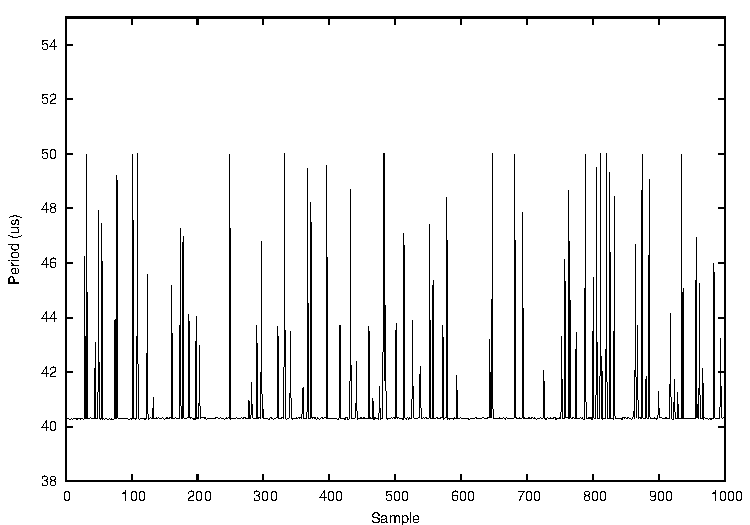
\includegraphics[scale=0.48]{interference_periodic_1000hz} &
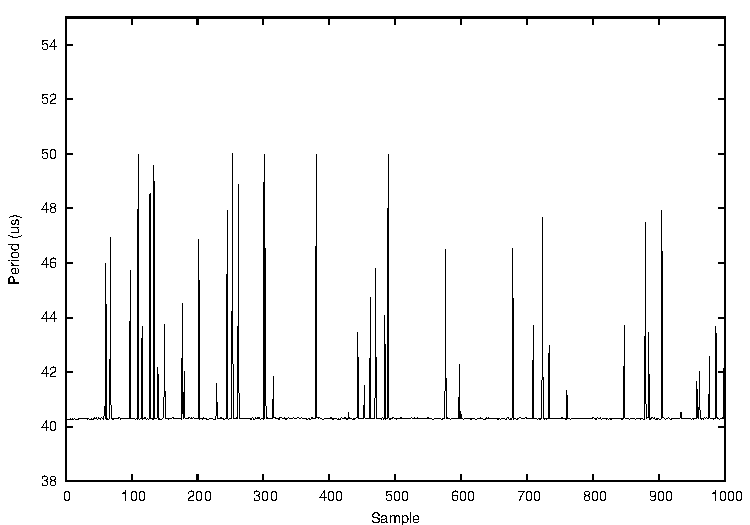
\includegraphics[scale=0.48]{interference_periodic_500hz}\\
(a) Periodic timer at 1000Hz & (b) Periodic timer at 500Hz\\
\\
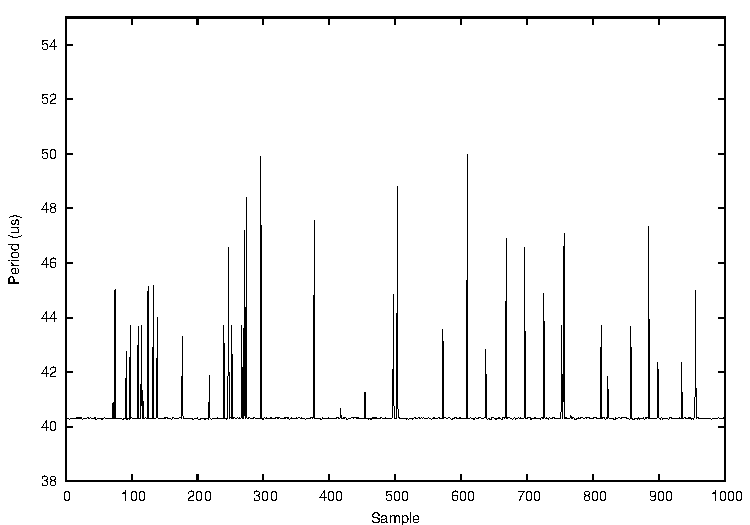
\includegraphics[scale=0.48]{interference_periodic_50hz} &
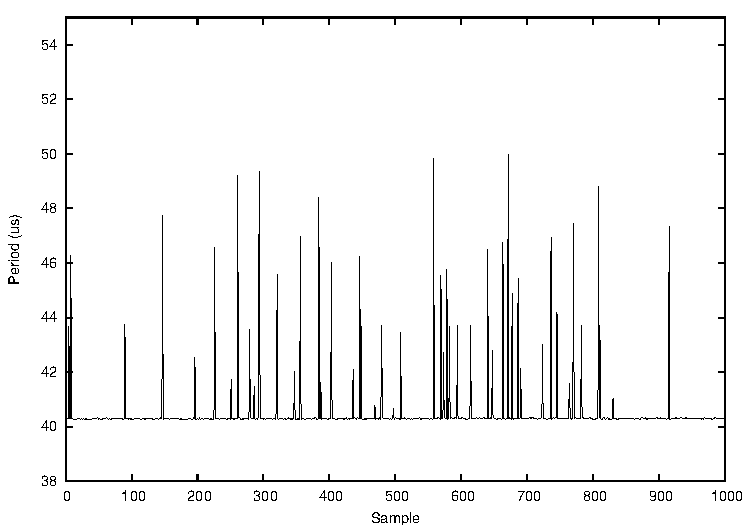
\includegraphics[scale=0.48]{interference_single-shot} \\
(c) Periodic timer at 50Hz & (d) Single-shot \\
\end{tabular}
\caption{Timer interference on the PWM thread's period along the time: (a)
  using periodic timer configured with 1000~Hz; (b) periodic timer with
  500~Hz; (c) periodic timer with 50~Hz; and (d) using single-shot
  timer.}
\label{fig:interference}
\end{figure*}

Figure~\ref{fig:deviation} summarizes the interference caused by timers
mechanisms on the period of the PWM thread in terms of standard
deviation. When the single-shot timer was used, the thread's average
period was 40.52~\us{}, with a standard deviation of 1.12~\us{} (2.77\%
of the thread's average period). When the 1000~Hz periodic timer was
used, the average period of this thread was 40.75~\us{} with a standard
deviation of 1.72~\us{} (4.23\% of the thread's average period). Since
the periodic timer is not well configured, it generates interrupts that
interfere with application.  On the other hand, the periodic timers
configured with 500~Hz and 50~Hz presented average periods of
40.51~\us{} and 40.44~\us{} respectively, but the 500~Hz periodic timer
obtained a higher standard deviation (1.19~\us{} of the thread's average
period).  Since the 50~Hz periodic timer will only generate interrupts
when necessary, it presented the best average period and standard
deviation (40.44~\us{} and 0.97~\us{}). This example shows how a bad
periodic timer configuration can affect the system performance.

\fig[ht]{deviation}{Mean period and standard deviation for each timer
  strategy and configuration with relation to
  Figure~\ref{fig:interference}.}{scale=0.6}

Our last experiment was designed to evaluate the performance of both
approaches in a scenario with concurrent time events. The objective is
to measure the execution time of the periodic interrupt handler in a
multi-threaded environment.  Figure~\ref{prg:threads_app} shows the
application used in this test.  The main function creates threads which
execute functions (\textit{func\_a}, \textit{func\_b}, etc). When the
alarm triggers, the thread is resumed (as described in
section~\ref{sec:design}) and repeats the loop. We ran this experiment
in the same AVR platform. Due to memory restriction, we only vary the
number of threads from 2 to 6. All threads have the same priority and
their periods were 10~\ms{}, 30~\ms{}, 60~\ms{}, 90~\ms{}, 120~\ms{},
and 150~\ms{} respectively. The hardware timer was configured with a
frequency of 100~Hz (period equal to 10~\ms{}) and clock frequency of
28800~Hz.

\begin{figure}[ht]
   \lstset{frame=single,language=C++,xleftmargin=2em,style=prg,basicstyle=\scriptsize}
   \begin{lstlisting}
Thread *a,*b,*c,*d,*e,*f;
int func_a() {
    while(1) { a->suspend(); /* suspends itself */ }
}
int func_b() {
    while(1) { b->suspend(); }
}
int main() {
    //creates all Threads and their Handlers
    a = new Thread(&func_a); Handler_Thread handler_a(a);
    b = new Thread(&func_b); Handler_Thread handler_b(b);
    ....
    //creates all Alarms
    Alarm alarm_a(Period_A, &handler_a, Alarm::INFINITE);
    Alarm alarm_b(Period_B, &handler_b, Alarm::INFINITE);
    ....
    int status_a = a->join(); int status_b = b->join();
    ....
}
   \end{lstlisting}
  \caption{Threads application test.}
  \label{prg:threads_app}
\end{figure}

For this test, we have changed the periodic timer interrupt handler in
order to release all time events which have their ticks less or equal to
zero in the same interrupt handler. Figure~\ref{fig:periodic_handler}
exemplifies the new interrupt handler scenario. It is important to
highlight that the timer job ends when it releases all threads. The
execution order of threads is guaranteed by the thread's priority in the
scheduler. In this case, the execution time of an interrupt handler is
not constant, it varies depending on the number of threads that reached
their period in that interrupt.

\fig[ht]{periodic_handler}{Periodic timer interrupt handler in a
  multi-threaded scenario. Note that the interrupt handler has different
  execution times.}{scale=.6}

Table~\ref{tab:thread_test} shows the periodic interrupt handler
execution time for this application varying the number of threads. When
running the application with 2 threads with periods of 10~\ms{} and
30~\ms{}, for instance, the average execution time was 81~\us{}, the
worst-case execution time was 111~\us{}, the best execution time was
63~\us{}, and the standard deviation was 23~\us{}. In comparison with
the single-shot interrupt handler execution time in
Table~\ref{tab:handler_time}, the periodic interrupt handler presented a
better performance up to 5 threads. With 6 threads, the worst-case
execution time of the periodic handler (263~\us{}) was worse than
single-shot (202~\us{}).

\begin{table}[ht]
\centering
\scriptsize{
\begin{tabular}{c|c|c|c|c}
\textbf{Number of}	& \multicolumn{4}{c}{\textbf{Interrupt Handling Time (us)}} \\
\cline{2-5}
\textbf{Threads}	& \textbf{Average}	& \textbf{Max} 	& \textbf{Min} & \textbf{Std} \\
\hline
\textbf{2} & 81  & 111   & 63   & 23 \\
\textbf{3} & 84  & 117   & 63   & 25 \\
\textbf{4} & 91  & 178   & 63   & 36 \\
\textbf{5} & 97  & 190   & 63   & 41 \\
\textbf{6} & 107 & 263   & 63   & 55 \\
\end{tabular}
}
\caption{Periodic timer interrupt handling time of the Threads application varying the number of threads.}
\label{tab:thread_test}
\end{table}

Two final remarks about the experiments carried out:

\begin{itemize}
\item Deeply embedded system

  Our work is focused on deeply embedded systems. Such systems present
  serious resources limitations, such as power consumption, processing
  power, and memory. Moreover, these systems are designed to run a
  specific set of applications, whose requirements are known at
  design-time. Therefore, configuring the periodic timer to fit system
  needs is a fully valid approach.

  Furthermore, the time spent by reprogramming the hardware timer in the
  single-shot implementation in a deeply embedded system is high, since
  this task involves calculations, like divisions and multiplications,
  in order to adjust the next time requested by the application to the
  hardware timer period.

\item \textsc{Epos} dependency

  The experiments described here used the \textsc{Epos} system, but the
  basic idea can be applied to virtually any embedded operating system.
  The problem itself is related to how the periodic timer is implemented
  and not to the embedded operating system. A smart periodic time
  management implementation can supply and adjust to the needs of
  embedded or real-time applications.

\end{itemize}

%------------------------------------------------------------------------ 
% 345 words - should be about 300
\section{Conclusion}\label{sec:con}

Common sense dictates that single-shot timer mechanisms are better than
periodic ones. Nonetheless, our experiments have shown that, for
real-time embedded systems, a properly configured periodic timer can
usually match the single-shot approach in terms of performance and
interference. This apparently unaccountable outcome arises basically
from the intrinsically periodic nature of embedded systems and from the
way timers are implemented in such systems. Indeed, the experiments have
shown that a periodic timer can outperform an equivalent single-shot
mechanism when the requested period exceeds the maximum hardware period
and the single-shot timer falls back to software tick counting. In this
case, the overhead of reprogramming the single-shot timer exceeds the
overhead of counting ticks. Moreover, in a multi-threaded environment,
the periodic interrupt handler presented better performance (up to 5
threads) in comparison to the single-shot interrupt handler using an
8-bit AVR microcontroller. This proves that the overhead of
reprogramming the hardware timer device must be consider by the
real-time embedded system designer.

A periodic timer mechanism does not require the hardware timer to be
reprogrammed for each event. The hardware timer is programmed during
system initialization to trigger interrupts with a frequency that best
matches the periods of events that will be handled by that system. This,
in combination with a properly designed event queue, can render a
simple, fast, and regular timer interrupt handler.  Furthermore, a
single-shot timer is limited by hardware resolution, and must fall back
to software tick counting when its resolution is exceeded.

Although this scenario of tailored periodic timer mechanisms does not
fit the all-purpose essence of ordinary OS, which must work in a
best-effort to accommodate a myriad of application demands, it does fit
well in the realm of real-time embedded systems. It is not our
intention, however, to promote periodic timers as a generally better
alternative for such systems than single-shot.  There are many cases in
the literature for which single-shot approaches have proved superior, in
particular, concerning power efficiency and jitter. Our main intention
is to reestablish periodic timer mechanisms as a concrete alternative
for real-time embedded systems.

\section*{Acknowledgment}\label{sec:ack}

We would like to thank and acknowledge LISHA members Lucas Wanner,
Roberto de Matos, and Danillo Moura Santos for the work on the initial
implementation of single-shot timers for \textsc{Epos} and for the
assistance with the experiments reported in this paper. We would also
like to thank Prof. R\^{o}mulo de Oliveira for the prolific discussions
about timing in real-time systems.


%% References
%%
%% Following citation commands can be used in the body text:
%% Usage of \cite is as follows:
%%   \cite{key}          ==>>  [#]
%%   \cite[chap. 2]{key} ==>>  [#, chap. 2]
%%   \citet{key}         ==>>  Author [#]

%% References with bibTeX database:

\bibliographystyle{model1-num-names}
\bibliography{timing}

%% Authors are advised to submit their bibtex database files. They are
%% requested to list a bibtex style file in the manuscript if they do
%% not want to use model1-num-names.bst.

%\section*{Authors' Biography}

\begin{description}
\item \textbf{Ant\^{o}nio Augusto Fr\"{o}hlich} is currently an
  Associate Professor for Operating Systems at UFSC. He received his PhD
  from the Technical University of Berlin in 2001. As Head of UFSC's
  Software/Hardware Integration Lab, he has led a number of R\&D
  projects on embedded systems. Since 2009 he leads a consortium to
  develop an Open, Free, Scalable Digital TV Platform.  \linebreak

\item \textbf{Giovani Gracioli} is a PhD student in Automation and
  Systems Engineering at UFSC. He received the Bachelor degree in
  Computer Science from the Federal University of Santa Maria in 2007
  and the Master degree in Computer Science from UFSC in 2009. His
  research areas include embedded, operating, and real-time systems.
  \linebreak

\item \textbf{Jo\~{a}o Felipe Santos} is a final year student in
  Electrical Engineering at UFSC. His research areas include embedded
  systems and computer architecture.

\end{description}

\end{document}

%%
%% End of file `elsarticle-template-1-num.tex'.
